\subsection[Konfiguracja urządzenia wykonującego]{Konfiguracja urządzenia wykonującego}
Uzyskanie zamierzonego efektu wymaga odpowiedniego oprogramowania i skonfigurowania urządzenia wykonującego.
Wszystkie urządzenia wykonujące przynależące do \textit{BSc-pen\-tes\-tera} działają pod kontrolą dedykowanej dla platformy \textit{Raspberry Pi} dystrybucji systemu Linux.
Umożliwia to sprawdzenie problemu konfiguracji do skorzystania z istniejących interfejsów jądra systemu, służących do tworzenia tzw. gadżetów USB. 
Termin gadżet USB używany jest do określenia urządzenia posiadającego własny kontroler urządzenia USB \textit{(ang. USB device controller, UDC)} oraz możliwość podłączenia do hosta USB w celu udostępnienia mu pewnych dodatkowych funkcjonalności.
Skonfigurowane w ten sposób urządzenie rozpoznawane jest przez hosta jako zbiór konfiguracji, z których każda zawiera pewne interfejsy (nazywane też funkcjami).
System Linux dostarcza wielu gotowych funkcji urządzeń USB np. obsługę wspomnianego w rozdziale~\ref{chapter:keyboard_mechanics} protokołu HID.
Realizowana konfiguracja korzysta z interfejsu USB Gadget Configfs, który pozwala na definiowanie konfiguracji i funkcjonalności złożonych gadżetów USB, czyli mogących udostępniać więcej niż jedną funkcjonalność - rysunek~\ref{fig:usbcompose}.
\begin{figure}[H]
    \centering
    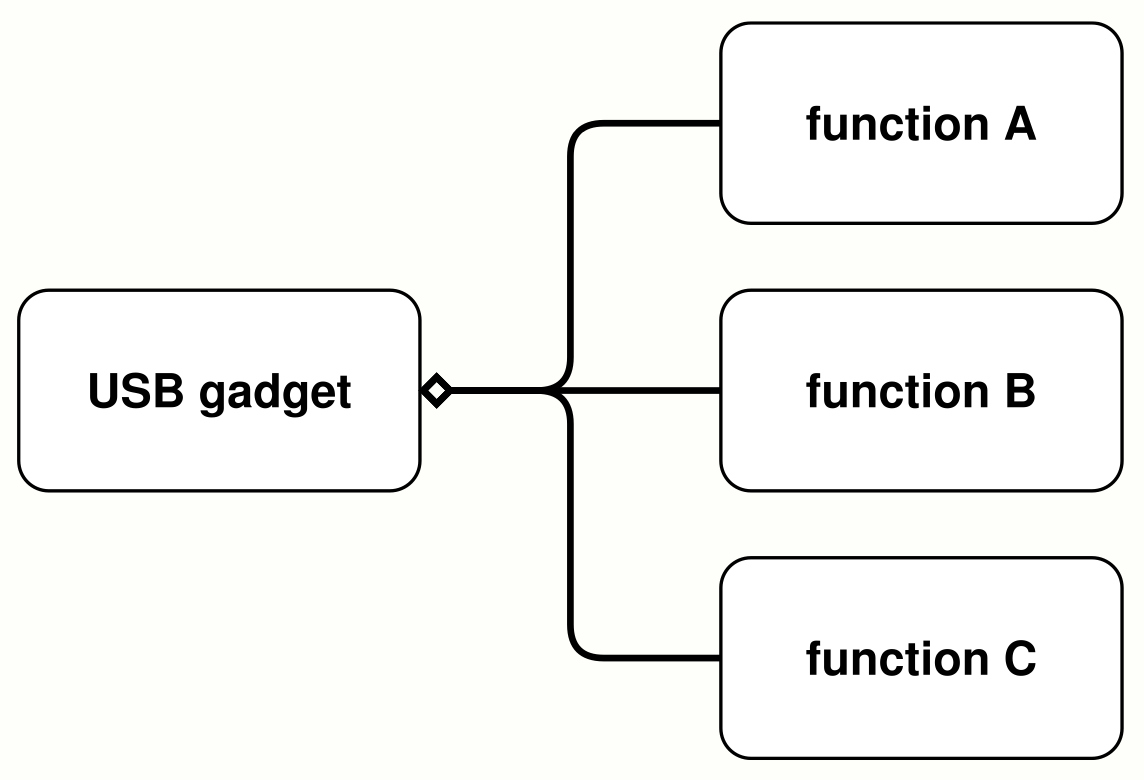
\includegraphics[width=0.5\textwidth]{images/usbcompose.png}
    \caption{Kompozycja gadżetu USB~\cite{samsung}}
    \label{fig:usbcompose}
\end{figure}
\noindent Proces przebiega z poziomu przestrzeni adresowej użytkownika~\cite{linaro}. Nie wymaga on realizacji własnych modułów jądra~\cite{samsung}. Mechanizm działania interfejsu Configfs ilustruje rysunek~\ref{fig:configfs}.
\begin{figure}[H]
    \centering
    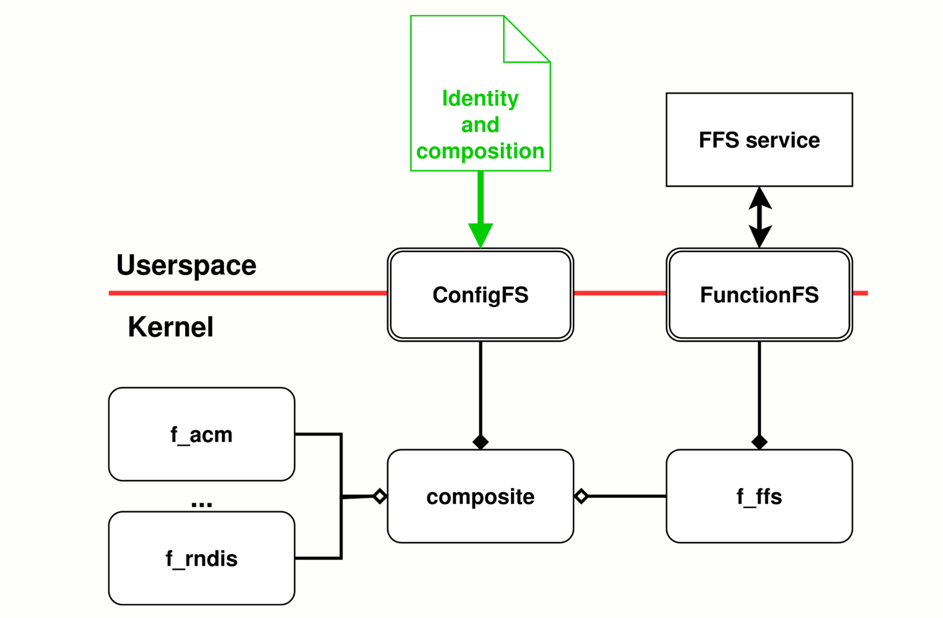
\includegraphics[width=0.8\textwidth]{mk01}
    \caption{Mechanizm działania configfs~\cite{samsung}}
    \label{fig:configfs}
\end{figure}
\noindent Do aktywacji interfejsu należy załadować dodatkowy modułu jądra oraz zamontować dedykowany system plików.
Można to zrobić prostymi poleceniami przedstawionymi w listnigu~\ref{lst:libcomposite}.
\begin{lstlisting}[language=bash,label={lst:libcomposite},caption={Inicjalizacja obsługi USB gadget configfs}]
    sudo modprobe libcomposite
    sudo mount none -t configfs /sys/kernel/config
\end{lstlisting}
\noindent Proces kreowania nowego urządzenia polega na wykonaniu operacji na plikach w nowo zamontowanym katalogu~\cite{samsung}.
Mapowanie akcji przedstawia tabela~\ref{tab:configs_map}.
\begin{table}[H]
    \begin{tabular}{|l|r|}
        \hline
        \textbf{Akcja} & \textbf{Operacja na systemie plików} \\
        \hline
            Stworzenie gadżet/funkcję/konfigurację & Stworzenie katalogu \textit{(mkdir)}\\
        \hline
            Usunięcie gadżet/funkcję/konfigurację & Usunięcie katalogu \textit{(rmdir)}\\
        \hline
            Ustawienie wartość atrybutu & Zapis do pliku \textit{(echo)}\\
        \hline
            Pobranie wartości atrybutu & Odczyt zawartości pliku \textit{(cat)}\\
        \hline
            Grupowanie funkcjonalności & Dowiązanie symboliczne \textit{(ln -s)}\\
        \hline
            Usunięcie grupy funkcjonalności & Usunięcie dowiązania symbolicznego \textit{(rm)}\\
        \hline    
    \end{tabular}
    \caption{Mapowanie operacji usb gadget configfs}  
    \label{tab:configs_map}
\end{table}
\noindent Następnym etapem konfiguracji jest zdefiniowanie nowego urządzenia po przez:
\begin{itemize}
    \item określenie identyfikatora urządzenia
    \item określenie identyfikatora dostawcy
    \item określenie realizowanych funkcjonalności.
\end{itemize}
Podstawowe elementy konfiguracji przedstawia listing~\ref{lst:usbconfig}
\begin{lstlisting}[language=python,label={lst:usbconfig},caption={Kreowanie urządzenia z poziomu języka python}]
import os

path = "/sys/kernel/config/usb_gadget/"
# definiowanie podstawowych informacji o urządzeniu
with open(os.path.join(path, "idVendor"), 'w') as file:
    file.write("0x1d6b")    # 0x1d6b => Linux Foundation

with open(os.path.join(path, "idProduct"), 'w') as file:
    file.write("0x0104")    # 0x0104 => Multifunction Composite Gadget

with open(os.path.join(path, "bcdDevice"), 'w') as file:
    file.write("0x0100")    # wersja urządzenia 1.0

with open(os.path.join(path, "bcdUSB"), 'w') as file:
    file.write("0x0200")    # maksymalna wspierana wersja standardu USB to 2.0

path = "/sys/kernel/config/usb_gadget/strings/0x409"    # ścieżka zawierająca stałe tekstowe

os.makedirs(path, exist_ok=True)

with open(os.path.join(path, "serialnumber"), 'w') as file:
    file.write("fedcba9876543210")  # przykładowy numer seryjny

with open(os.path.join(path, "manufacturer"), 'w') as file:
    file.write("BSC")   # tekst reprezentujący 'producenta'

with open(os.path.join(path, "product"), 'w') as file:
    file.write("BSC") # tekst reprezentujący nazwę produktu

os.makedirs("/sys/kernel/config/usb_gadget/configs/c.1", exist_ok=True)

# definiowanie funkcjonalności HID
path = "/sys/kernel/config/usb_gadget/functions/hid.usb0"
os.makedirs(path, exist_ok=True)

with open(os.path.join(path, "protocol"), 'w') as file:
    file.write("1")

with open(os.path.join(path, "subclass"), 'w') as file:
    file.write("1")

with open(os.path.join(path, "report_length"), 'w') as file:
    file.write("8")

with open(os.path.join(path, "report_desc"), 'wb') as file:
    file.write(binarnie_zakodowany_deskryptor)  # deskryptor HID omawiany w rozdziale~\ref{chapter:keyboard_mechanics}

os.symlink(path, "/sys/kernel/config/usb_gadget/configs/c.1/hid.usb0")

# finalizacja
path = "/sys/kernel/config/usb_gadget/"
with open(os.path.join(path, "UDC"), 'w') as file:
    file.write('\n'.join(os.listdir("/sys/class/udc")))
\end{lstlisting}
Po tak przygotowanej konfiguracji i podłączeniu urządzenia wykonującego, proces wysyłania raportu odbywa się przez zapis jego bajtów do pliku \textit{/dev/hidg0}. 

